\section{Installation instructions}
The following software are needed

\begin{itemize}
\item MySql Community Server  5.7.24 or MySql Community Server 8.0.13
\item MySql Connector/J 5.1.47
\item MySql Workbench 8.0.13 (Optional)
\item JDK 8 Update 144
\item Glassfish 5.0
\end{itemize}




\subsection{Database initialization}
After having installed MySql Server, you have to create the database for trackme.
In the repository you can find 3 sql file to do this:

\begin{enumerate}
\item \texttt{create.sql}
\item \texttt{sample.sql}
\item \texttt{bigsample.sql}
\end{enumerate}
As their name suggest, the first one create the database and the tables, the second populated the tables with some small data, while the last one insert a larger, randomly generated, amount of data.
Notice that running any of these files will drop the existing data currently stored in the database.
\vspace{1em}

\noindent 
In order to execute those sql you can type in the terminal

\begin{center}
\texttt{mysql -u your\_username -p \textless\ you\_file.sql}
\end{center}
and enter your password.
Alternatively, you can use MySql Workbench with \textit{File/Run sql script}.


\subsection{Connection pool configuration}
Assuming \textit{domain1} is in use on glassfish, copy \texttt{mysql-connector-java-5.1.47-bin.jar} in the folder

\begin{center}
glassfish5/glassfish/domains/domain1/lib 
\end{center}
Now follow the next steps.
\begin{enumerate}
\item Start glassfish server.
\item Open the administration panel (usually on port 4848).
\item Select \textit{Resources/JDBC/JDBC Connection Pools} on the tree on the left.
\item Click \textit{New..}.
\item In the \textit{Pool Name} field enter \texttt{TrackmePool}.
\item As \textit{Resource Type} select \texttt{javax.sql.DataSource}.
\item As \textit{Database Driver Vendor} select \texttt{MySql}.
\item Click \textit{Next}.
\item Make sure that \textit{Data Source Classname} is \texttt{com.mysql.jdbc.jdbc2.optional.MysqlDataSource}.
\item In \textit{Additional Properties}, you can delete all the default ones and set the following:
	\begin{itemize}
	\item \texttt{portNumber}: the port of your mysql server, usually \texttt{3306};
	\item \texttt{user}: your username for the mysql server;
	\item	\texttt{password}: your password for the mysql server;
	\item \texttt{databaseName}: enter the value \texttt{trackme} as defined in the SQL DD.
	\end{itemize}
\item Click \texttt{Finish}.
\end{enumerate}

Now your database connection pool should be configured, you can check selecting the connection pool and clicking \textit{Ping} (be sure that the MySql server is running).
A \textit{Ping Succeeded} message should show up.\vspace{1em}


\noindent
In order to allow the application to use this connection pool, a new JNDI resource must be created.
From the glassfish administration panel:

\begin{enumerate}
\item Select \textit{Resources/JDBC/JDBC Resources} on the tree on the left.
\item Click \textit{New..}.
\item As \textit{JNDI Name} enter \texttt{jdbc/trackme} (note that this name is important, if different the application will not be able to locate the resource).
\item As \textit{Pool Name} select the \texttt{TrackmePool} just created.
\item Click \textit{OK}.
\end{enumerate}


\subsection{Certificate issue for Nominatim API}
It can happen that the call the to Nominatim API fails due to certification issue.
This problem can be noted in the Glassfish log file when trying to perform a call for a location coordinates.
If the problem is not fixed, the location constraints for group data request are simply ignored.
\vspace{1em}

\noindent
A possible fix is to use the certificates distributed along with the JDK 8.
From the installation folder of the JDK, go to Contents/Home/jre/lib/security and copy the \texttt{cacerts} file.
Go to the Glassfish installaton folder and then, assuming domain1 is in use, to glassfish/domains/domain1/config.
Here there should be an already exiting \texttt{cacerts.jks}, replace this file with the previously copied from the JDK (adding the extension could be necessary).




\subsection{Web App Deployment}
After downloaded the \texttt{trackme.war} from the repository, follow the next steps in order to deploy the application. Be sure that the mysql server is running and the connection pool properly configured.

\begin{enumerate}
\item Start glassfish server.
\item Open the administration panel (usually on port 4848).
\item Select \textit{Applications} on the tree on the left.
\item If not already selected, select \textit{Packaged File to Be Uploaded to the Server} and choose the \texttt{trackme.war} previously downloaded.
\item In the \textit{Contex Root} field enter \texttt{trackme}.
\item Click \textit{OK}.
\end{enumerate}
Now the trackme server should have been correctly deployed, to verify this, go to
\begin{center} http://localhost:8080/trackme/login.xhtml\end{center}
the login page (or the homepage if the browser sent a valid authentication cookie) should appear.

\subsection{Android App deployment}

To install the app on your android phone first enable the installation from unknown sources. Then download the app from the delivery folder in your phone, find it with a file manager and tap on it. Allow the installation and wait for the process to finish. The app should now have been installed.

\begin{center}
   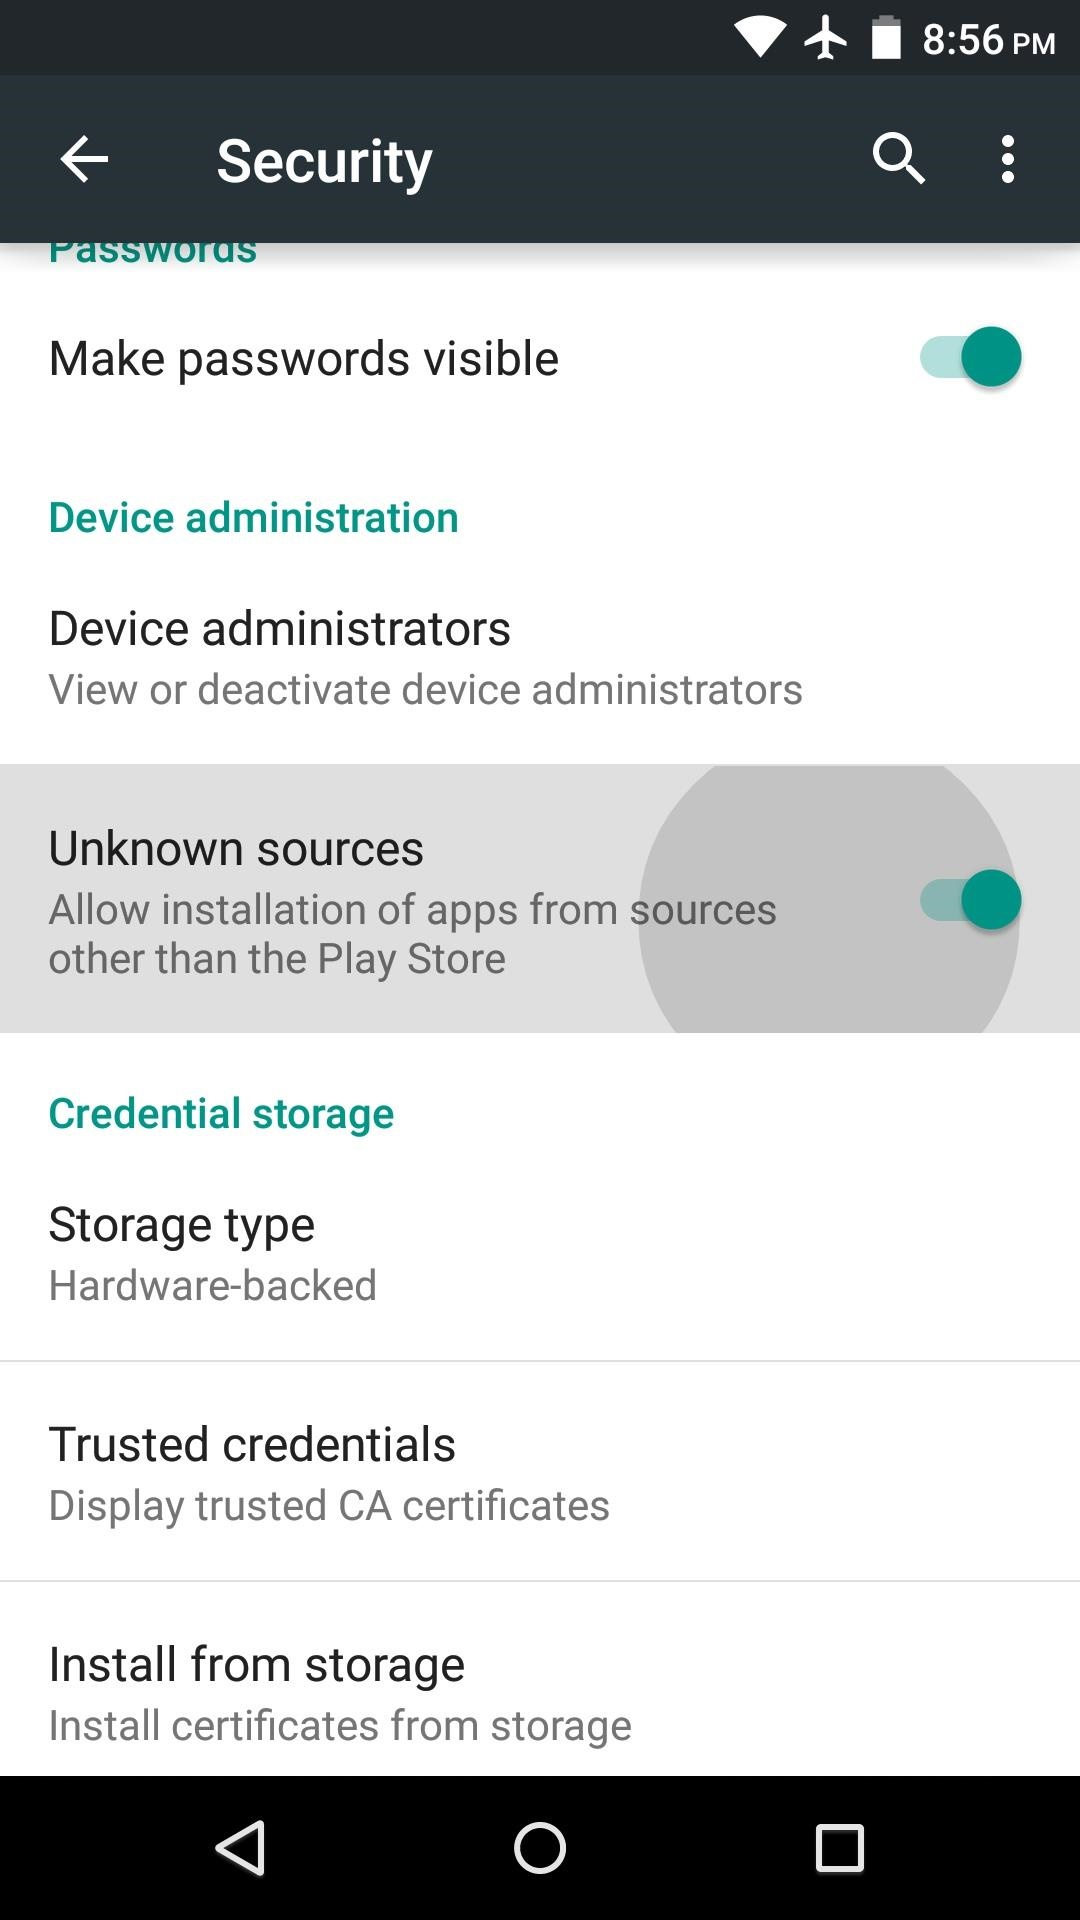
\includegraphics[scale=0.15]{resources/unknowsources.jpg}
   \captionof{figure}{Unknown sources screen}
\end{center}


Alternatively the app can be installed on an android studio emulator, that comes bundled with android studio.
First thing that is necessary to deploy the app on your emulator is to have ADB installed in your system. Mind that each OS has its own version of ADB, so make sure to install the correct one.
Next download the app and move it to android\textbackslash{}sdk\textbackslash{}tools or platform-tools folder. The path to these folders changes based on the OS.
Open the terminal and go to the folder containing the apk then execute the following command:
adb install apkname.apk.
The apk should now have been installed.

Note: In case of multiple emulator error, run the command adb devices, pick the id of your emulator (it is usually emulator-5554) and then run the command adb -s <your emulator id> install <apk name> from the folder where the apk was moved before.


\subsection{Setting up the App}

By tapping more than 10 times on the App logo in the main screen the user can have access to the developer screen.


\begin{center}
   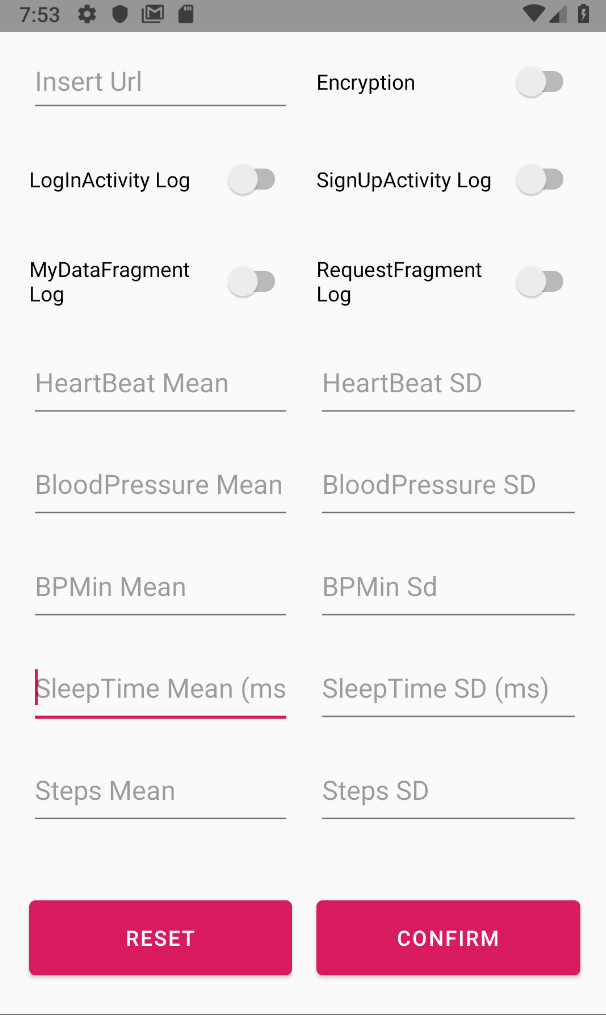
\includegraphics[scale=0.5]{resources/developerscreen.png}
   \captionof{figure}{Developer Screen screenshot}
\end{center}



As can be seen from the image various settings can be specified, but the most important is the serverl url: by default the url provided bundled with the apk is the one that lets the emulator connect to the localhost. Of course this cannot be used if the App has been launched on the phone, so in the Url text field it should be specified the host url of the server. This corresponds  to http://ipv4netip:8080/trackme/rest/ in the case that both the smartphone and the device running the server are under the same network, where the ipv4netip is the network ip of the machine that runs the server.
Moreover, to use the preloaded individual tuples that come with the DB, the encryption should be disables (it is disabled by default) since that the password contained in the DB are not hashed.
In the end some other parameters like activating various log for the activities, or setting up the parameters for the gaussian distribution for each data can be set.
To apply the changes tap on the confirm button.
In the end remember that this choices are kept as long as they are not cleared by tapping on the reset button in the developer screen.



